\section{stack}
% \par \noindent 给出一个01矩阵,求全1子矩阵的个数。

\par \noindent Xác định ma trận 01 và tìm số ma trận con có các phần tử bằng 1.

\begin{enumerate}
% \item 按行枚举子矩阵的底边,然后求以该行为底边的子矩阵的个数。
\item Liệt kê các cơ số của các ma trận con theo hàng, sau đó tìm số ma trận con có cơ số của hàng đó.
% \item 预处理 int H[N][N]:向上最大扩展全1的长度,然后就可以用单调栈解决。
\item Tiền xử lý int H[N][N]: Mở rộng lên tới độ dài tối đa của cả 1 và sau đó có thể giải quyết bằng ngăn xếp đơn điệu.
% \item 为了避免计算重复,单调栈时左闭右开即可。
\item Để tránh tính toán lặp lại, ngăn xếp đơn điệu có thể được đóng ở bên trái và mở ở bên phải.
\end{enumerate}

\begin{figure}
        \centering
        \par 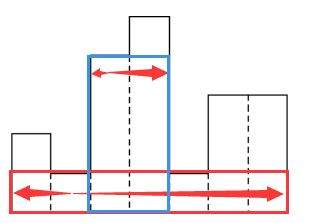
\includegraphics[width=10cm]{images/stack.png}
\end{figure}

% \par \noindent 按照上述思想也能够求最大子矩形的面积。
\par \noindent Theo ý tưởng trên cũng có thể tìm được diện tích của hình chữ nhật phụ lớn nhất.
~\\
% \par \noindent 注意此做法能够优化到O(矩形1的数量),因为可以直接枚举同一行的1的位置,考虑该行相邻列都是1的情况此时计算一次答案。【按照矩形的分布计算,因为一个位置是0就可以隔断子矩形】

\par \noindent Lưu ý rằng phương pháp này có thể được tối ưu hóa thành O (số hình chữ nhật 1), vì vị trí của các số 1 trong cùng một hàng có thể được liệt kê trực tiếp và câu trả lời được tính toán khi xem xét rằng các cột liền kề của hàng đều là 1. [Tính theo phân bố của hình chữ nhật, vì vị trí 0 có thể tách hình chữ nhật phụ]

\begin{minted}{c++}
#include <bits/stdc++.h>

using namespace std;

const int N = 1e3 + 5;
using ll    = int64_t;
int n, m, a[N][N];
int H[N][N]; 

ll calc(int* h, int k) { // Tính số hình chữ nhật chỉ số [0, k)
    stack<int> s;
    vector<int> l(k), r(k);
    for (int  i = k - 1; i >= 0; i--) {
        while (!s.empty() && h[i] <= h[s.top()]) l[s.top()] = i, s.pop();
        s.push(i);
    }
    while (!s.empty()) l[s.top()] = -1, s.pop();
    
    for (int  i = 0; i <= k - 1; i++) {
        while (!s.empty() && h[i] < h[s.top()]) r[s.top()] = i, s.pop();
        s.push(i);
    }
    while (!s.empty()) r[s.top()] = k, s.pop();
    ll res = 0;
    for (int  i = 0; i <= k - 1; i++)  res += (ll)h[i] * (i - l[i]) * (r[i] - i);
    return res;
}

int main() {
    scanf("%d%d", &n, &m);
    for (int i = 1; i <= n; i++) 
        for (int j = 1; j <= m; j++) 
            scanf("%d", &a[i][j]);
    ll ans = 0;
    
    for (int i = 1; i <= n; i++)  {
        for (int j = 1; j <= m; j++) {
            if (a[i][j])
                H[i][j] = H[i-1][j] + 1;
            else
                H[i][j] = 0;
        }
        ans += calc(H[i] + 1, m); // Đếm một lần mỗi hàng
    }
    
    printf("%lld\n", ans);
    return 0;
}
/**
2 2
0 1
1 1 
Số hình chữ nhật con là 5
**/
\end{minted}